% ####
% CAPA
% ####

% ----
% Informações da Capa
% ----
\newcommand{\capatitulo}{
\vphantom{espaço vertical em branco}
Documentação

Projeto Sistema \emph{DNC}
}

\newcommand{\capasubtitulo}{
%\large Notas da Reunião do dia 09 de Agosto de 2021 

\large Autor: Ronie Paulucio Porfirio

\vphantom{\small Publicado no DCL nº 22, de 16 de março de 2021}
}

\newcommand{\capaunidade}{
\large Eu

\Large Eu

\vphantom{espaço vertical em branco}
}

% ----
% Código  
% ----
\begingroup

\thispagestyle{empty} % Suppress headers and footers on the title page

\begin{tikzpicture}[remember picture,overlay]
\node[inner sep=0pt] (background) at (current page.center) 
{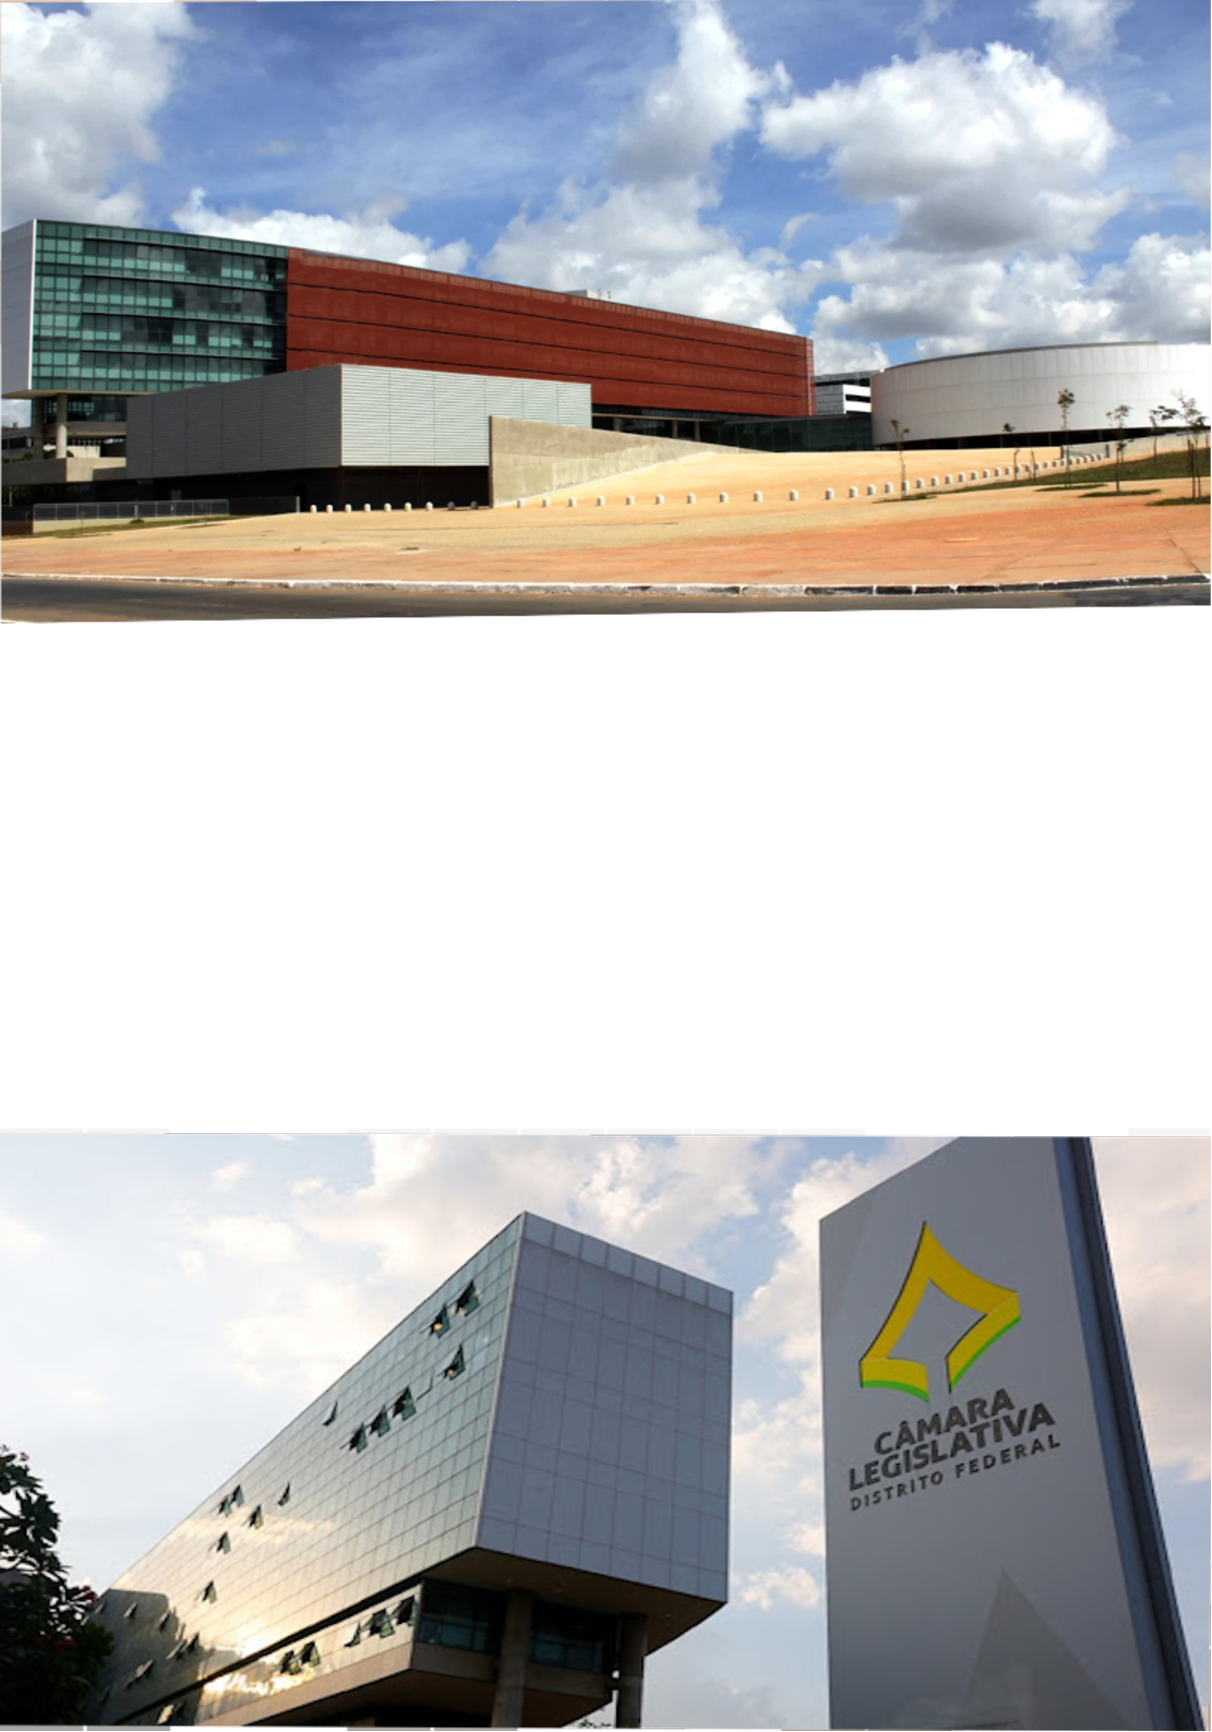
\includegraphics[width=\paperwidth]{capa.pdf}};
\draw (current page.center) node [fill=ocre!30!white,fill opacity=0.8,text opacity=1,inner sep=1cm]{\Huge\centering\bfseries\sffamily\parbox[c][][t]
{\paperwidth}
{
\centering \capatitulo\\[15pt] % Book title
{\Large \capasubtitulo}\\[20pt] % Subtitle
{\capaunidade} % Author name
}}; 
\end{tikzpicture}

\vfill

\endgroup
